% Version 1.2 of SN LaTeX, November 2022
%
% See section 11 of the User Manual for version history 
%
%%%%%%%%%%%%%%%%%%%%%%%%%%%%%%%%%%%%%%%%%%%%%%%%%%%%%%%%%%%%%%%%%%%%%%
%%                                                                 %%
%% Please do not use \input{...} to include other tex files.       %%
%% Submit your LaTeX manuscript as one .tex document.              %%
%%                                                                 %%
%% All additional figures and files should be attached             %%
%% separately and not embedded in the \TeX\ document itself.       %%
%%                                                                 %%
%%%%%%%%%%%%%%%%%%%%%%%%%%%%%%%%%%%%%%%%%%%%%%%%%%%%%%%%%%%%%%%%%%%%%

%%\documentclass[referee,sn-basic]{sn-jnl}% referee option is meant for double line spacing

%%=======================================================%%
%% to print line numbers in the margin use lineno option %%
%%=======================================================%%

%%\documentclass[lineno,sn-basic]{sn-jnl}% Basic Springer Nature Reference Style/Chemistry Reference Style

%%======================================================%%
%% to compile with pdflatex/xelatex use pdflatex option %%
%%======================================================%%

%%\documentclass[pdflatex,sn-basic]{sn-jnl}% Basic Springer Nature Reference Style/Chemistry Reference Style


%%Note: the following reference styles support Namedate and Numbered referencing. By default the style follows the most common style. To switch between the options you can add or remove “Numbered” in the optional parenthesis. 
%%The option is available for: sn-basic.bst, sn-vancouver.bst, sn-chicago.bst, sn-mathphys.bst. %  
 
%%\documentclass[sn-nature]{sn-jnl}% Style for submissions to Nature Portfolio journals
%%\documentclass[sn-basic]{sn-jnl}% Basic Springer Nature Reference Style/Chemistry Reference Style
\documentclass[sn-mathphys,Numbered]{sn-jnl}% Math and Physical Sciences Reference Style
%%\documentclass[sn-aps]{sn-jnl}% American Physical Society (APS) Reference Style
%%\documentclass[sn-vancouver,Numbered]{sn-jnl}% Vancouver Reference Style
%%\documentclass[sn-apa]{sn-jnl}% APA Reference Style 
%%\documentclass[sn-chicago]{sn-jnl}% Chicago-based Humanities Reference Style
%%\documentclass[default]{sn-jnl}% Default
%%\documentclass[default,iicol]{sn-jnl}% Default with double column layout

%%%% Standard Packages
%%<additional latex packages if required can be included here>

\usepackage{graphicx}%
\usepackage{multirow}%
\usepackage{amsmath,amssymb,amsfonts}%
\usepackage{amsthm}%
\usepackage{mathrsfs}%
\usepackage[title]{appendix}%
\usepackage{xcolor}%
\usepackage{textcomp}%
\usepackage{manyfoot}%
\usepackage{booktabs}%
\usepackage{algorithm}%
\usepackage{algorithmicx}%
\usepackage{algpseudocode}%
\usepackage{listings}%
%%%%
%\usepackage{caption}

%%%%%=============================================================================%%%%
%%%%  Remarks: This template is provided to aid authors with the preparation
%%%%  of original research articles intended for submission to journals published 
%%%%  by Springer Nature. The guidance has been prepared in partnership with 
%%%%  production teams to conform to Springer Nature technical requirements. 
%%%%  Editorial and presentation requirements differ among journal portfolios and 
%%%%  research disciplines. You may find sections in this template are irrelevant 
%%%%  to your work and are empowered to omit any such section if allowed by the 
%%%%  journal you intend to submit to. The submission guidelines and policies 
%%%%  of the journal take precedence. A detailed User Manual is available in the 
%%%%  template package for technical guidance.
%%%%%=============================================================================%%%%

%\jyear{2021}%

%% as per the requirement new theorem styles can be included as shown below
\theoremstyle{thmstyleone}%
\newtheorem{theorem}{Theorem}%  meant for continuous numbers
%%\newtheorem{theorem}{Theorem}[section]% meant for sectionwise numbers
%% optional argument [theorem] produces theorem numbering sequence instead of independent numbers for Proposition
\newtheorem{proposition}[theorem]{Proposition}% 
%%\newtheorem{proposition}{Proposition}% to get separate numbers for theorem and proposition etc.

\theoremstyle{thmstyletwo}%
\newtheorem{example}{Example}%
\newtheorem{remark}{Remark}%

\theoremstyle{thmstylethree}%
\newtheorem{definition}{Definition}%

\raggedbottom
%%\unnumbered% uncomment this for unnumbered level heads

\begin{document}

%\title[Article Title]{Developing Comprehensive Annotation Guidelines and a Corpus of Risk of Bias Assessment for Rehabilitation: A Methodological Approach}
\title[Article Title]{RoBuster: A Validation Corpus with Risk of Bias span annotations in Randomized Controlled Trials}

%%=============================================================%%
%% Prefix	-> \pfx{Dr}
%% GivenName	-> \fnm{Joergen W.}
%% Particle	-> \spfx{van der} -> surname prefix
%% FamilyName	-> \sur{Ploeg}
%% Suffix	-> \sfx{IV}
%% NatureName	-> \tanm{Poet Laureate} -> Title after name
%% Degrees	-> \dgr{MSc, PhD}
%% \author*[1,2]{\pfx{Dr} \fnm{Joergen W.} \spfx{van der} \sur{Ploeg} \sfx{IV} \tanm{Poet Laureate} 
%%                 \dgr{MSc, PhD}}\email{iauthor@gmail.com}
%%=============================================================%%

\author*[1,2]{\fnm{Anjani} \sur{Dhrangadhariya}}\email{anjani.dhrangadhariya@hevs.ch}

\author[3]{\fnm{Roger} \sur{Hilfiker}}\email{roger.hilfiker@proton.me}

\author[4]{\fnm{Martin} \sur{Sattelmayer}}\email{martin.sattelmayer@hevs.ch}

\author[5,6]{\fnm{Nona} \sur{Naderi}}\email{nona.naderi@hesge.ch}

\author[4]{\fnm{Katia} \sur{Giacomino}}\email{katia.giacomino@hevs.ch}
\equalcont{These authors contributed equally to this work.}

\author[4]{\fnm{Rahel} \sur{Caliesch}}\email{rahel.caliesch@hevs.ch}
\equalcont{These authors contributed equally to this work.}

\author[1,2]{\fnm{Henning} \sur{Müller}}\email{henning.mueller@hevs.ch}


\affil*[1]{\orgdiv{Department of Computer Science}, \orgname{University of Geneva}, \orgaddress{\city{Geneva}, \country{Switzerland}}}

\affil[2]{\orgdiv{Informatics Institute}, \orgname{HES-SO Valais-Wallis}, \orgaddress{\city{Sierre}, \country{Switzerland}}}

\affil[3]{\orgdiv{IUFRS}, \orgname{University of Lausanne}, \orgaddress{\city{Lausanne}, \country{Switzerland}}}

\affil[4]{\orgdiv{School of Health Sciences}, \orgname{HES-SO Valais-Wallis}, \orgaddress{\city{Leukerbad}, \country{Switzerland}}}

\affil[5]{\orgdiv{Geneva School of Business Administration}, \orgname{HES-SO Geneva}, \orgaddress{\city{Geneva}, \country{Switzerland}}}

\affil[6]{\orgname{Swiss Institute of Bioinformatics (SIB)}, \orgaddress{\city{Geneva}, \country{Switzerland}}}

%%==================================%%
%% sample for unstructured abstract %%
%%==================================%%

\abstract{The abstract serves both as a general introduction to the topic and as a brief, non-technical summary of the main results and their implications. Authors are advised to check the author instructions for the journal they are submitting to for word limits and if structural elements like subheadings, citations, or equations are permitted.}

%%================================%%
%% Sample for structured abstract %%
%%================================%%

% \abstract{\textbf{Purpose:} The abstract serves both as a general introduction to the topic and as a brief, non-technical summary of the main results and their implications. The abstract must not include subheadings (unless expressly permitted in the journal's Instructions to Authors), equations or citations. As a guide the abstract should not exceed 200 words. Most journals do not set a hard limit however authors are advised to check the author instructions for the journal they are submitting to.
% 
% \textbf{Methods:} The abstract serves both as a general introduction to the topic and as a brief, non-technical summary of the main results and their implications. The abstract must not include subheadings (unless expressly permitted in the journal's Instructions to Authors), equations or citations. As a guide the abstract should not exceed 200 words. Most journals do not set a hard limit however authors are advised to check the author instructions for the journal they are submitting to.
% 
% \textbf{Results:} The abstract serves both as a general introduction to the topic and as a brief, non-technical summary of the main results and their implications. The abstract must not include subheadings (unless expressly permitted in the journal's Instructions to Authors), equations or citations. As a guide the abstract should not exceed 200 words. Most journals do not set a hard limit however authors are advised to check the author instructions for the journal they are submitting to.
% 
% \textbf{Conclusion:} The abstract serves both as a general introduction to the topic and as a brief, non-technical summary of the main results and their implications. The abstract must not include subheadings (unless expressly permitted in the journal's Instructions to Authors), equations or citations. As a guide the abstract should not exceed 200 words. Most journals do not set a hard limit however authors are advised to check the author instructions for the journal they are submitting to.}

\keywords{risk of bias, data annotation, natural language processing, large language models}

%%\pacs[JEL Classification]{D8, H51}

%%\pacs[MSC Classification]{35A01, 65L10, 65L12, 65L20, 65L70}

\maketitle


%%%%%%%%%%%%%%%%
%% Background %%
\section{Background and Significance}
\label{sec:background}
%
Systematic reviews (SRs) synthesized using randomized controlled trials (RCTs) are the highest quality of evidence in the evidence pyramid.
SRs aid medical professionals make educated decisions about an individual's health and help governments enact informed health policies~\cite{mogo2022systematic,mctigue2006obesity}.
An RCT is a scientific experiment aiming to evaluate the efficacy of an intervention on particular patient outcomes.
In these trials, patients are randomly divided and allocated to either an active intervention group or a comparator group, and the impact of intervention compared to the comparator is measured in a controlled setting~\cite{sibbald1998understanding}.
Theoretically, RCTs are less susceptible to biases given the randomized study design but are still prone to unavoidable flaws in the trial's design, conduction, or reporting.
Biased clinical trials make medical practitioners systematically overestimate or underestimate the intervention effect on patient outcomes, leading to harmful health practices and policies~\cite{kjaergard1999randomized,naci2019design}.
Thus, Reviewers conducting SRs must thoroughly screen RCTs for biases before inclusion in writing SRs.


The biases in RCTs cannot be quantified, but an RCT can be assessed for biases to minimize the overall risk and judge its quality.
Various terms are used for bias assessment, like validity or quality assessment, but in this study, we refer to bias assessment as risk-of-bias (RoB) assessment.
There are several tools to assess RoB, including the Cochrane Collaborations RoB Tool, Physiotherapy Evidence Database (PEDro) RoB scale, revised Cochrane RoB 2.0 tool, AMSTAR/AMSTAR 2, EPOC RoB Tool and several other independent checklists~\cite{higgins2011cochrane,elkins2013growth,sterne2019rob,shea2017amstar,farrah2019risk}.
These tools are structured as a series of questions aiming to elicit factual information from the RCTs, which could then be used for RoB assessment.
%These tools are a series of questions aiming to elicit factual information from the RCTs, which can then be used to assess their quality.
Manual quality assessment requires the reviewers to go through full-text RCTs and manually inspect every question from the chosen bias assessment tool.
The process takes about 3-10 months per person per SR and requires a high degree of methodological expertise on the reviewer's part.
Moreover, RoB assessment is a part of writing systematic reviews, which is highly resource-heavy, taking about six months to several years to complete~\cite{tsertsvadze2015conduct, khangura2012evidence}.
review~\cite{higgins2019cochrane}.
The pace at which RCTs are published makes RoB assessment a lengthy process and underscores the need for automation..
%~\footnote{\url{https://pubmed.ncbi.nlm.nih.gov/?term=randomized\%20controlled\%20trial&filter=pubt.randomizedcontrolledtrial}

Machine learning (ML) can help accelerate the assessment process by directly pointing the reviewers to the parts of the RCT text relevant to identifying bias, leading to quickly judging the trial quality.
Marshall \textit{et al.}~\cite{marshall2015automating} attempted automation of RoB assessment using distant supervision approach supported by proprietary data from the Cochrane Database of Systematic Reviews (CDSR). 
They formulated the trial quality assessment as binary classification into \textit{low-risk} and \textit{unclear-risk/high-risk} quality attributes for each risk domain.
The study was supported by the manually-entered data from CDSR, which is behind a paywall and automates based on Cochrane's RoB 1.0 guidelines and not the latest RoB 2.0~\cite{higgins2011cochrane}.
Even though Cochrane's RoB tool (version 1) is the most frequently used to assess RCT quality, a recently revised Cochrane RoB 2.0 offers significant differences in comparison~\cite{ma2020methodological}.
Compared to the original RoB version released in 2008, the 2.0 version provides a more reliable and concrete structure to the RoB evaluation by developing comprehensive guidelines that enforce consistency~\cite{higgins2011cochrane,sterne2019rob}.
A study analyzing Cochrane systematic reviews and protocols found that the use of RoB 2.0 increased from 0\% in 2019 to 24.1\% in 2022~\cite{martimbianco2023most}.
This indicates a growing recognition of the importance of using an updated and standardized tool to assess bias in RCTs.

Millard \textit{et al.} attempted automating RoB assessment using supervised machine learning trained on proprietary data as well~\cite{millard2016machine}.
In fact, the research utilising this pay-walled data was used to develop RobotReviewer that has been evaluated by several studies for its human-competent performance~\cite{marshall2016robotreviewer,soboczenski2019machine,vinkers2021methodological,jardim2022automating,hirt2021agreement}.
The question, however, remains of the unavailability of a publicly-available RoB annotated corpus that hinders community efforts for automation. 
Wang \textit{et al.} recently released three RoB annotated datasets, but for preclinical animal studies with RoB assessments pertaining to animals~\cite{wang2022risk}.
Manual RoB assessment is a complex, expert-led task laden with subjective judgements.
Systematically translating this manual process for developing an RoB annotated corpus requires a carefully designed annotation scheme and detailed annotation guidelines.
Recently Dhrangadhariya \textit{et al.} worked on a pilot study to test whether RoB 2.0 guidelines could be utilized as guidelines to manually annotate a corpus of randomized controlled trials with RoB using a multi-level annotation scheme adapted from the same guidelines.
They neither provide any annotation guidelines and their dataset is comparatively small with 10 annotated RCTs~\cite{dhrangadhariya2023first}.
Our objective is to develop clear cut annotation guidelines to annotate RCTs with RoB categories corresponding to RoB 2.0 tool for randomized trials~\cite{sterne2019rob}.



Recently, large language models (LLMs) have demonstrated exceptional performance on unseen tasks when only the task instructions are provided~\cite{chang2023survey}.
However, till date, no one has evaluated their performance on the cognitively complex task of identifying RoB text descriptions from RCTs and providing their risk judgments based on text.
Our contributions with this paper are five-fold. 
1) We develop comprehensive annotation guidelines for annotating RCTs with risk of bias description.
2) We model these annotation guidelines in form of visual placards for ease of annotation and understanding. These placards could be used as visual RoB assessment guidelines by the trainee RoB assessors.
3) We annotate a corpus of 60 full-text RCTs with more than 20 risk of bias span types which could be used to train machine learning models or LLMs and could also be used as a validation benchmark.
4) We evaluate the performance of LLMs to automatically identify the answers to these signalling questions using prompt generation.
5) We make the annotation guidelines, the dataset and LLM prompts openly-available for the scientific community.
%
%
%
\section{Methodology}
\label{sec:methods}
%
This section describes the annotation scheme, annotation softwares and guidelines.
Since there are no annotation guidelines available for RoB span annotation task, we take pleasure in formulating them from scratch. 
We first developed a draft version of our visual annotation guidelines, doubly annotated a fraction of documents using it and used this exercise to refine the guidelines.
%
%
%
\subsection{Annotation scheme}
\label{met:annot_scheme}
%

%
%
%
\begin{figure}
    \centering
    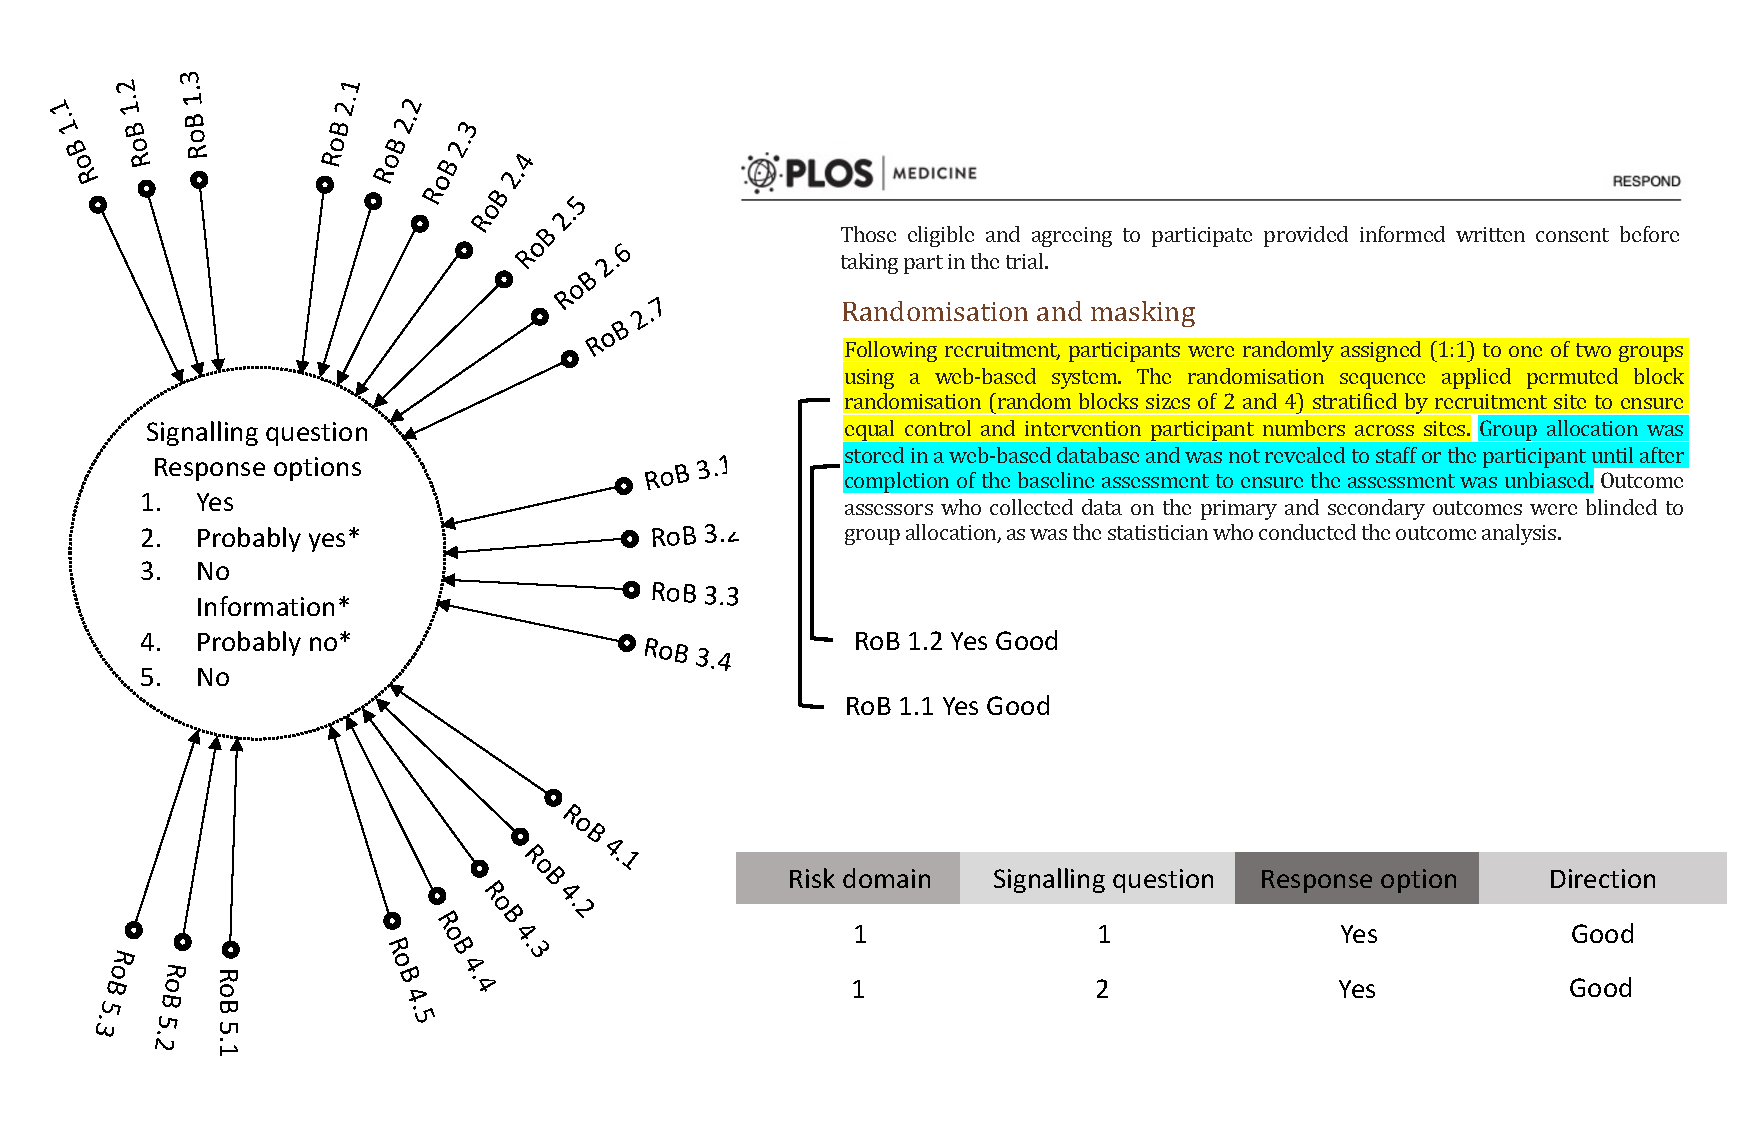
\includegraphics[width=0.99\columnwidth]{figures/annotation_schema.pdf}
    \caption{Our annotation scheme}
    \label{fig:annotationscheme}
\end{figure}
%
%
%



Creating a new annotated corpus involves defining an annotation scheme or adopting an existing one.
To our knowledge the only available annotation scheme for RoB span annotation was presented by ~\cite{dhrangadhariya2023first}.
Rather than creating a new scheme, we adapt and enhance their approach by learning from its drawbacks.
Their annotation scheme was directly adapted from the RoB 2.0 assessment procedure and hence it is imperative to understand the RoB 2.0 structure to understand the annotation scheme.
RoB 2.0 divides biases into five risk domains, each corresponding to different parts of the trial design.
Each risk domain decomposes into several signalling questions, each aiming to prompt a relevant response to bias assessment (refer to Table~\ref{tab1}).


%
%
%
\begin{table*}
 \centering
 %\captionsetup{justification=justified}
   \caption{The table lists down the bias domains as structured in the revised Cochrane RoB assessment tool (RoB 2.0) and the number of signalling questions (SQ) in each domain.}\label{tab1}
    \begin{tabular}{|l|l|r|}
    \hline
     Class & Domain & SQ\\
    \hline
    \hline
    RoB 1 & biases arising from the randomization process &  3\\
    RoB 2 & biases due to deviations from intended interventions & 7\\
    RoB 3 & bias due to missing outcome data & 4\\
    RoB 4 & bias in the measurement of the outcome & 5\\
    RoB 5 & bias in the selection of the reported result & 3\\
    \hline
    \end{tabular}
\end{table*}
%
%
%


The response options are restricted to ``Yes'', ``Probably yes'', ``No'', ``Probably no'', or ``No information''~\cite{sterne2019rob}.
Reviewers assess these signalling questions by examining the factual evidence in the RCT.
For instance, to answer the signalling question ``Was the allocation sequence random?'', the reviewer reads through the study to identify how participants were randomized into intervention groups.
If a well-executed method of randomization is identified, the reviewer answers with ``yes'' (the allocation sequence is random) judging the risk of bias for this signaling question as low risk.
Conversely, if a poorly executed method of randomization is found, the risk of bias is deemed  high risk with response option ``no''.
%Similarly, each signalling question prompts the reviewer to look for a piece(s) of factual evidence in the clinical study to respond with one of the five response options.



In RoB span annotation, we mimic this assessment process by considering evidence text spans in the RCT as the main units of annotation. 
Each span corresponds to answering a signalling question and is annotated with the most informative label. 
The label incorporates information about the signalling question number and the domain it assesses (for the above example, ``1.1'' for the first domain and first signalling question of the domain)
Additionally, the response judgement is incorporated in the label, such as ``1.1 Yes Good'' for a well-executed randomization (see Figure~\ref{fig:annotationscheme}).
Dhrangadhariya \textit{et al.} suggests collapsing the response options ``yes'' and ``probably yes'' into a single ``yes'', and ``no'' and ``probably no'' together into a single ``no'' to increase the inter-annotator agreement (IAA)~\cite{dhrangadhariya2023first}.
Except for some special case signalling questions, we too collapse these response option as suggested.
As shown in Figure~\ref{fig:flowchart} responding to any signalling question for the risk domain 2 as either ``Probably yes'' or ``Yes'' does not alter the final risk judgment for this domain (low, high, or some concerns).
In summary, the reviewer needs to label the identified text span with the RoB entity along with one of the response options.
In this regard, we have a hierarchical span annotation scheme comprising 22 entities corresponding to the 22 signalling questions, each with typically two response options and two directions (mutually exclusive).
We also remove the ``No Information'' labels since it is meant for the situations where actually no text evidence is found to answer a SQ leaving on text to be labelled with it.
However, for selected signalling questions, ``probably yes'', ``probably no'' and ``No Information'' may still be used.
For example, consider that an RCT uses ``...random number generator and sealed envelopes for patient randomization...'', but the trial provided no information on whether the envelop was ``opaque'' or not.
In such situations, ``No Information'' label is acceptable.
%Additionally, it is based on this span, the response judgment option is decided, and therefore even the response judgement information is incorporated in the label.
%Consider the following span is found to answer the above-mentioned signalling question, ``randomized participants using random number generation...'', which is a good randomization procedure and therefore the reviewer responds with ``yes''.
%The label extends the example label to ``1.1 Yes''.
%In addition, a direction is also added to the label, for example, whether it is ``good'' or ``bad.
%In this example, a good randomization ensure low risk for this signalling question and vice versa.
%Adding direction extends the example label to ``1.1 Yes Good''.


%
%
%
\begin{figure}
    \centering
    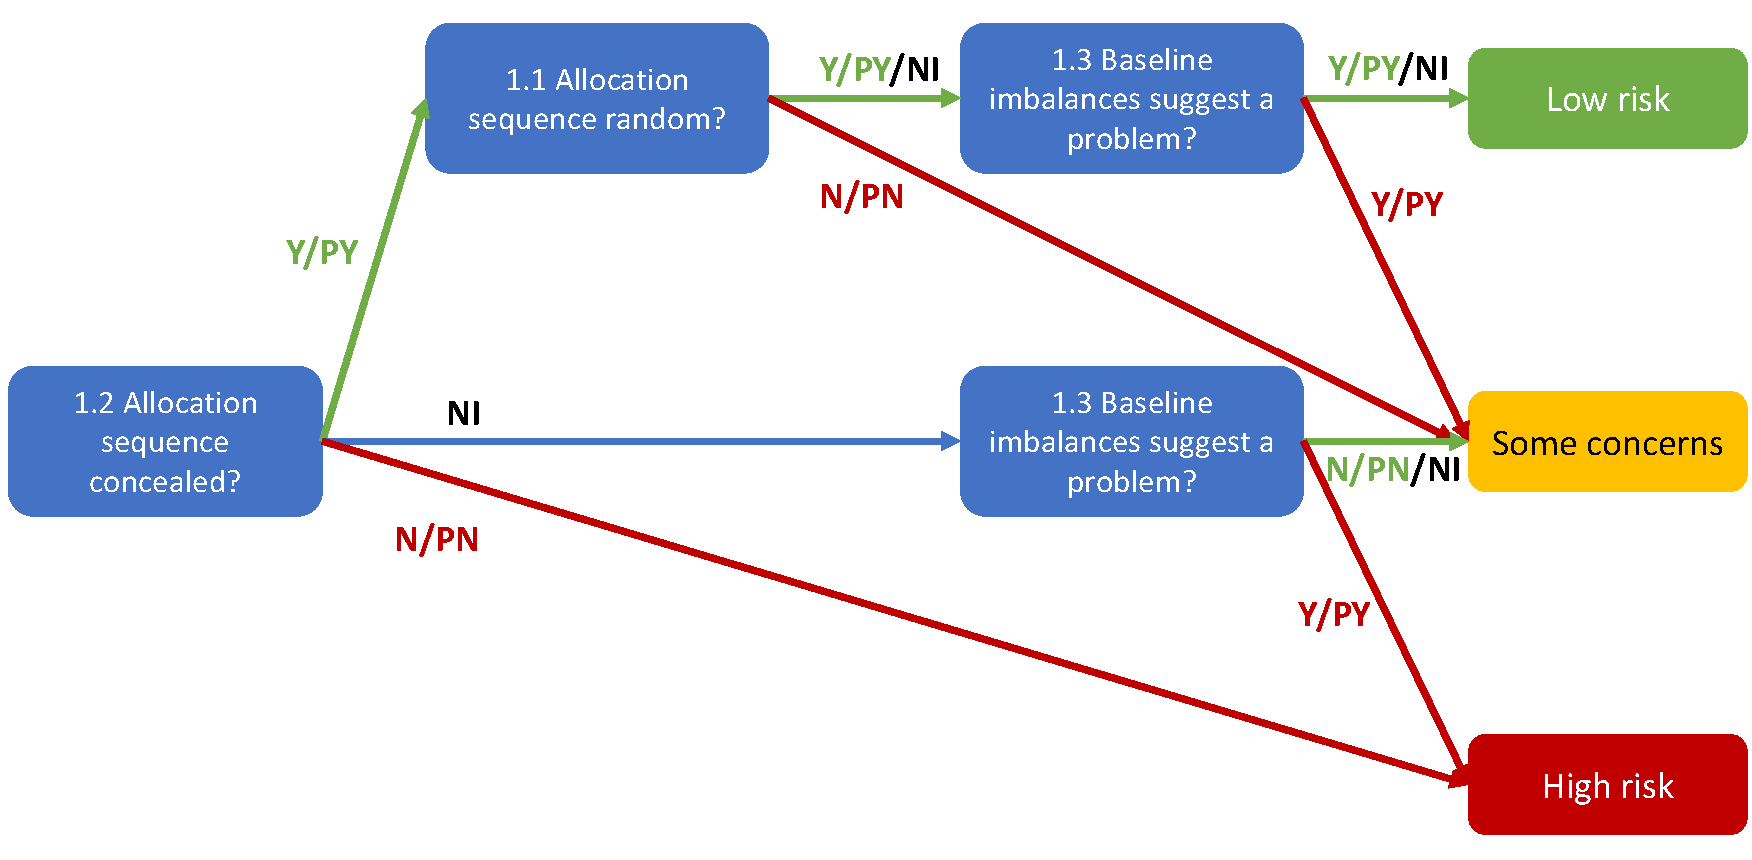
\includegraphics[width=0.60\columnwidth]{figures/flowchart.pdf}
    \caption{Algorithm for suggested judgement of risk of bias arising from the randomization process. Taken from the revised Cochrane's risk of bias tool (RoB 2.0).}
    \label{fig:flowchart}
\end{figure}
%
%
%

%
%
%
\subsection{Data collection}
\label{data}
%
The epidemiology researcher from our team created an annotation dataset of 60 RCTs from the domain of physiotherapy and rehabilitation.
Our corpus is focused on these domains because our annotators have RoB assessment expertise in this domain.
Savović~\textit{et al.} categorized outcome measures as mortality, other objective outcome, or subjective outcome and estimated the associations of bias judgments with intervention effect estimates~\cite{savovic2018association}.
Trials assessing subjective outcomes are more prone to bias, therefore, had we used only one outcome type, we would have limited label types for different risk classes~\cite{page2016empirical}.
In context of RCTs, subjective outcomes are measurements that rely on individuals' perceptions, opinions, or feelings about their own health or well-being.
These outcomes are typically self-reported by the participants in the trial and can be influenced by factors such as  placebo effects, patient expectations, interpretation, and psychological factors.
For example, in a study on rheumatoid arthritis, subjective outcome measures included patient-reported pain ratings~\cite{vollert2020assessment}.
Objective outcomes are measurements that are independent of individual opinions or perceptions and are based on observable and measurable data.
These outcomes are typically collected by trained assessors or through laboratory tests, imaging studies, or other objective methods.
For instance, in a study on peripheral artery disease, objective outcome measures included angiography and molecular imaging to evaluate the effectiveness of cell therapy~\cite{grimaldi2016imaging}.
Mortality outcomes refer to the occurrence of death during the course of the randomized controlled trial.
To ensure these different outcome types are represented in the corpus, we restricted including 26, 23 and 11 RCTs addressing objective, subjective and mortality primary outcomes.
These 60 studies were selected from four journals: journal 1, journal 2, journal 3 and journal 4. 
PDFs of the full-text RCTs were extracted and each article was collated with its trial protocol wherever available.
%TODO Anjani: Justify why only these journals were considered?
%TODO Anjani: Add if some studies were randomly added. Ask Roger for more information.
All these RCT PDFs have CC-BY-0 licences~\footnote{\url{https://creativecommons.org/share-your-work/public-domain/cc0/}}.
We list these studies and their licenses in the supplementary material.

%
%
%
%\begin{itemize}
%    \item 60 RCTs
%    \item Between 2001:2021
%    \item CC0, CC BY, CC BY non-commercial
%    \item Eutils search - Include search query for PubMed
%    \item Search for each year, retmax=not defined, randomly selected 20 studies from the retrieved
%    \item Take the first three studies with free-full text available.
%    \item Upload to tagtog
%\end{itemize}
%
%
%
\subsection{Expert team}
\label{experts}
%
As mentioned earlier, risk of bias annotation is a complex task that requires specialized expertise.
It's mentally demanding due to the need to carefully go through the entire full-text of RCTs and identify 22 different bias categories for annotation.
This level of task complexity would not be manageable for annotators without expertise in the field.
Our annotation team consisted of two researchers specializing in RoB assessment in physiotherapy and rehabilitation domains, including an epidemiology researcher and an assistant professor in physiotherapy.
With a substantial background in both physiotherapy, advanced statistical methods and experience writing systematic reviews, both experts possesses a deep understanding of the complexities involved in assessing bias risk in research studies.
Two additional physiotherapy experts, a post-doc and a senior PhD student, were a part of developing the visual annotation guidelines.


Additionally, two researchers with expertise in natural language processing (NLP) were involved, one being a computational linguistics professor and the other a PhD student in computer science.
The inclusion of NLP researchers was particularly important because the guidelines and placards they helped create will be utilized to annotate a text corpus, which will serve as a benchmark for the NLP task of RoB span extraction.
%
%
%
\subsection{Guideline development}
\label{guidelines}
%
%
%
%
\begin{figure}
    \centering
    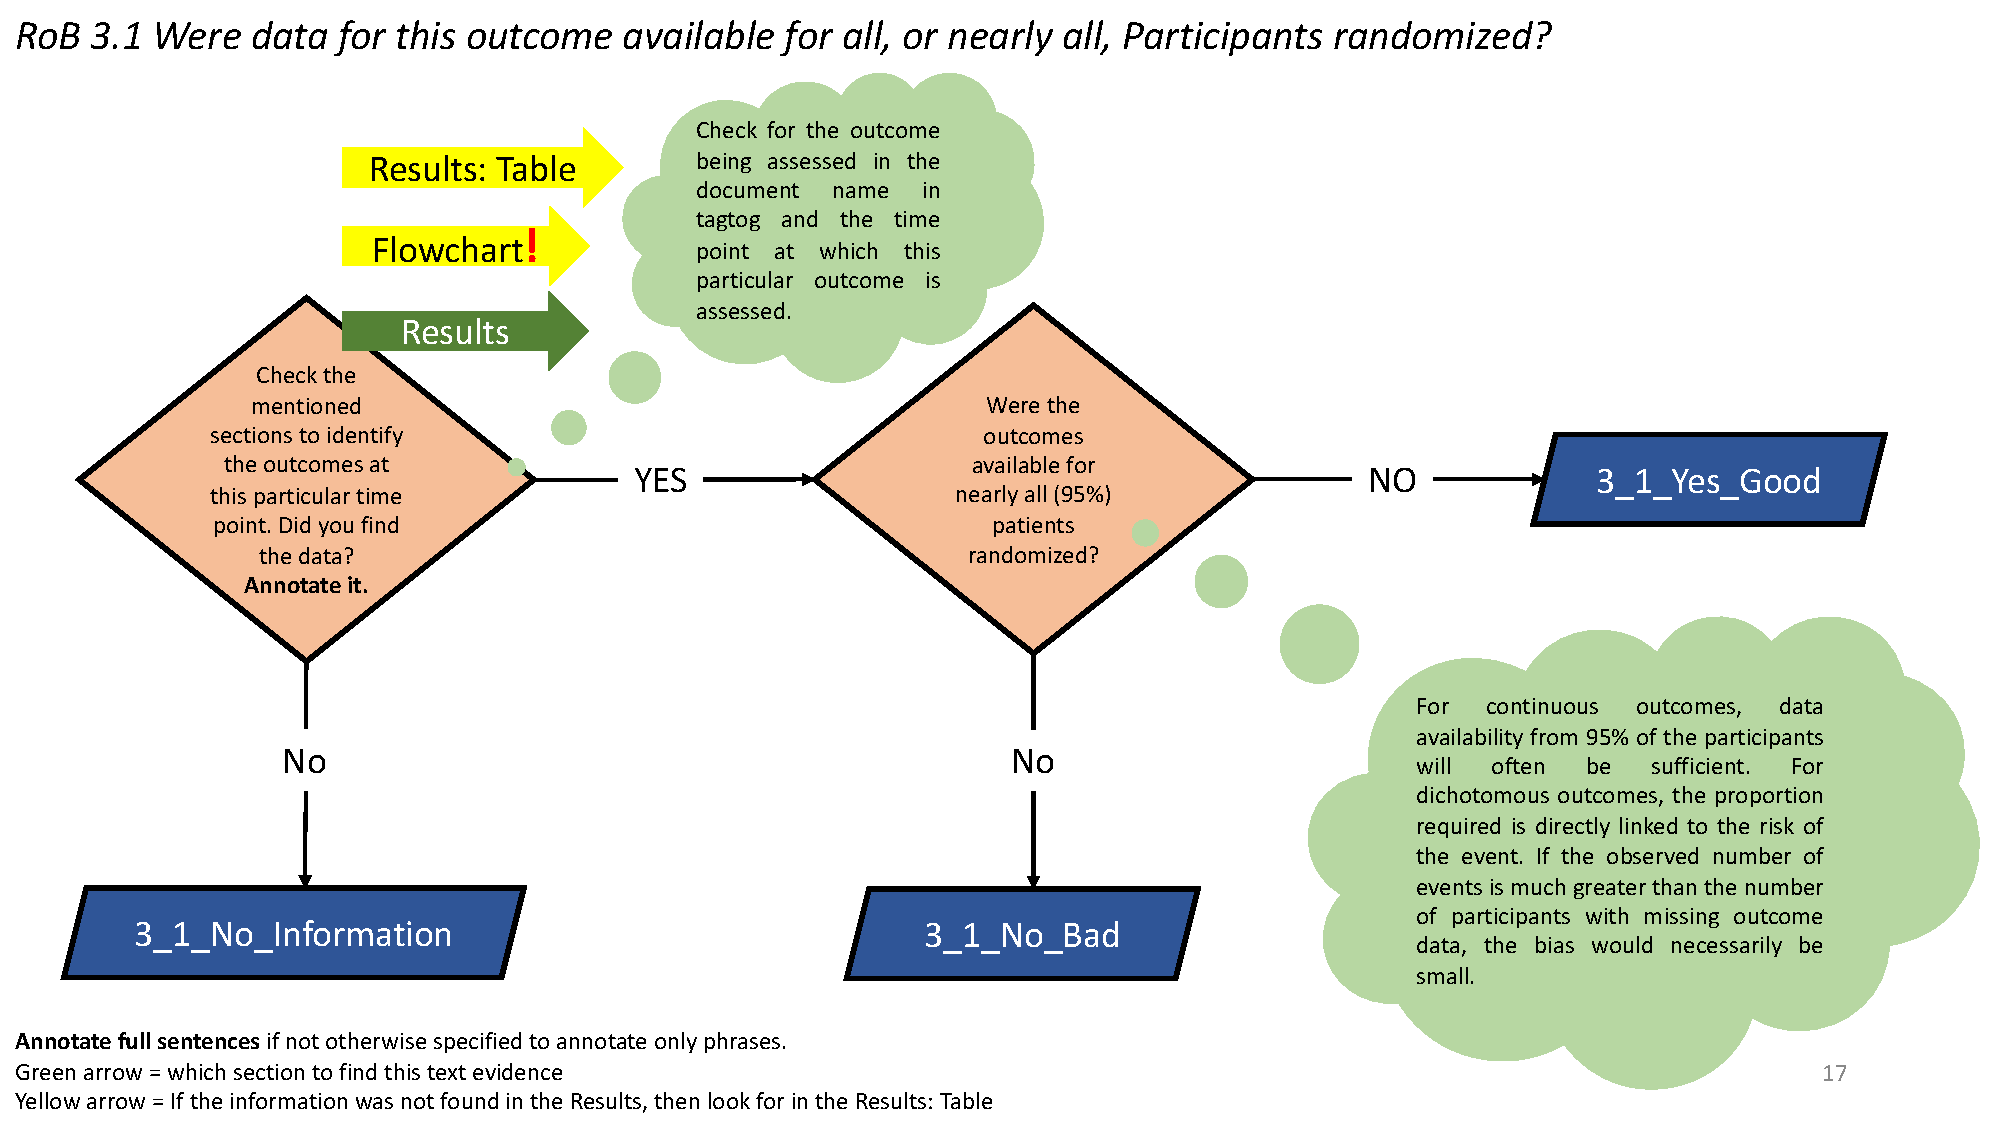
\includegraphics[width=0.80\columnwidth]{figures/placard_3_1.pdf}
    \caption{Example annotation instruction placard for the signalling question 3.1 from RoB 2.0 tool.}
    \label{fig:flowchart}
\end{figure}
%
%
%

RoB 2.0 guidelines consist of extensive and step-by-step set of instructions that utilize signaling questions, which are detailed in subsection~\ref{met:annot_scheme}.
Even though RoB 2.0 guidelines are widely used for bias assessment, there have been some research on the reliability of these guidelines.
This reliability concern of RoB 2.0 has been extensively investigated by Minozzi \textit{et al.}. 
They formulated specific instructions on how to approach and answer the signaling questions of RoB 2.0.
These instructions, referred to as the Instruction Document (ID), address the subjectivity present in the RoB 2.0 guidelines and provide clear guidance for the assessment process.
Subjectivity in assessment could potentially result in different evaluators coming to disparate conclusions when analyzing the same trial.
Before implementing the ID, the agreement among four expert RoB assessors was zero, but it improved after adopting the ID.
Several other papers explored subjectivity and reliability of the Cochrane RoB 1.0 and 2.0 tools~\cite{minozzi2022reliability,da2017effect,loef2022interrater,minozzi2020revised}.
%Anjani: Comments from Roger and Martin about the inherent subjectivity
%The signalling questions are broadly factual but leave room for subjective judgements and aim to facilitate judgements about the risk of bias.


Given the significance of maintaining consistency and reliability among annotators, we undertook the development of precise and clear annotation guidelines.
Working closely with our team of experts, we formatted these guidelines into visual placards.
Each placard takes the form of a flowchart and provides instructions for annotating a single signaling question.
These placards address various facets of RoB 2.0 subjectivity and the actual process of annotation.
For instance, a common reason for low inter-annotator agreement is when annotators correctly address a bias question but annotate evidence from different parts of the full text. 
To tackle this, our placards restrict annotations for a question to a specific part of the text, such as the Methods section, Results section, Flowchart in the Methods section, etc.
Detailed guidelines and these visual placards are available in the Supplementary material, with an example placard shown in the Figure.
These placards also tackle another factor contributing to the low inter-annotator agreement.
For example, while some annotators might annotate an entire paragraph as text evidence to answer a question, others might focus on the most informative portion of the text.
To address this, the placards provide clear guidance on whether annotators should annotate a phrase, a sentence, or a combination of sentences.
%
%
%
\subsection{Annotation}
\label{annotation}
%
%
%
%
\begin{figure}[htb]
    \centering
    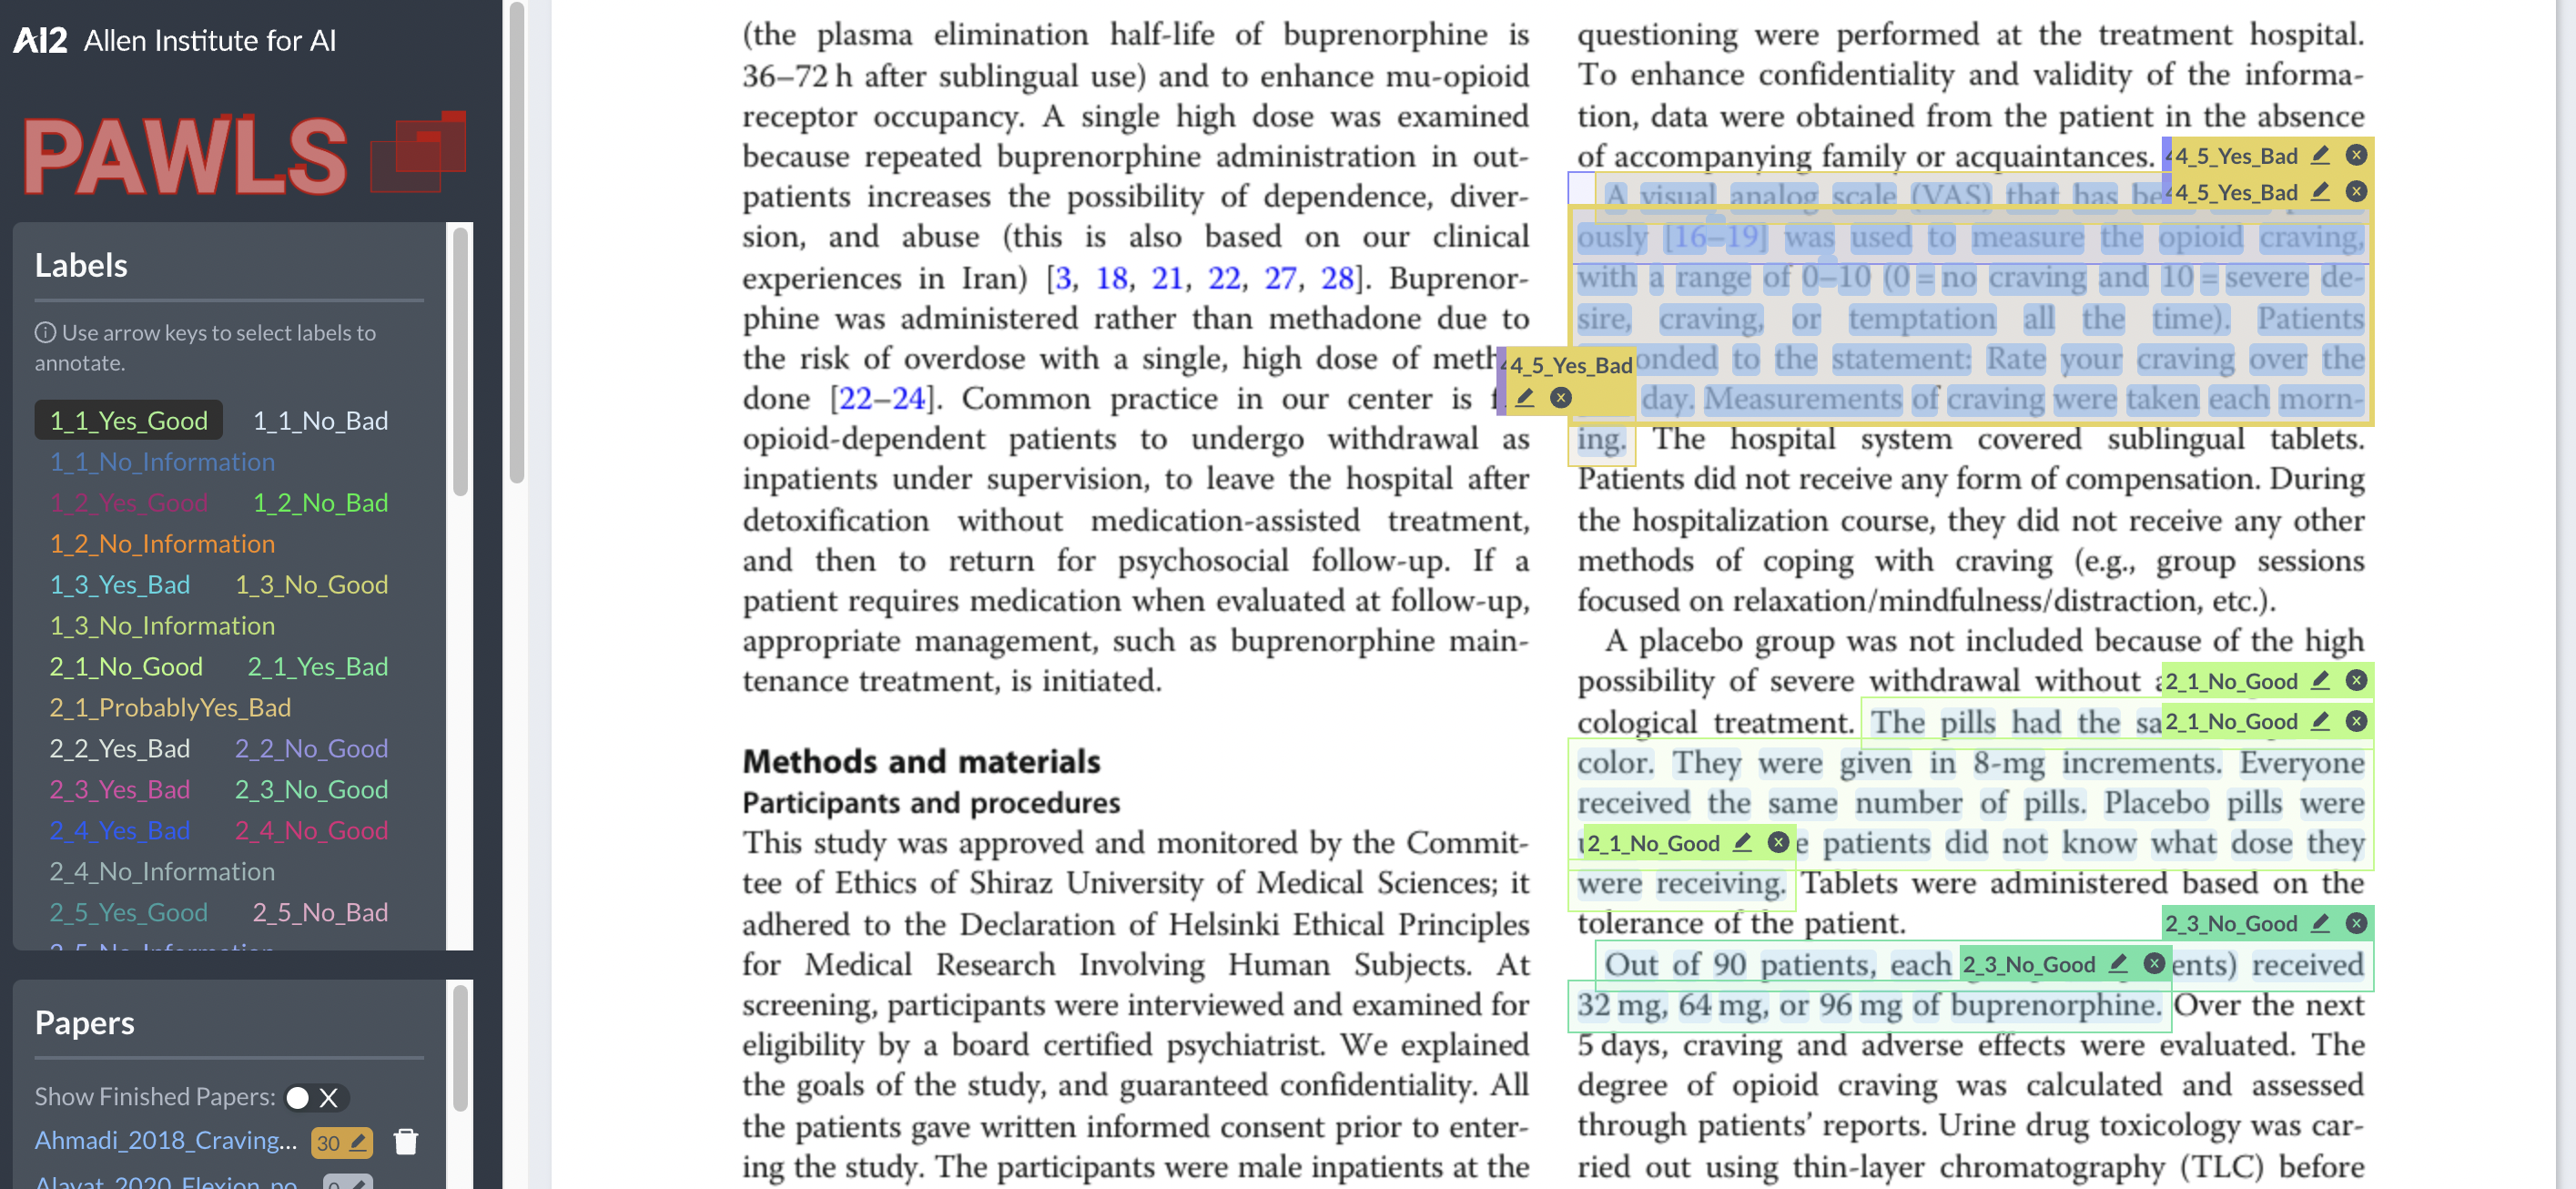
\includegraphics[width=0.80\columnwidth]{figures/pawls_layout.png}
    \caption{PAWLS layout example.}
    \label{fig:pawls}
\end{figure}
%
%
%

Tagtog~\footnote{\url{https://www.tagtog.net/}}, a commercial text annotation web application, allows for annotating PDF (Portable Document Format) documents, was used for the annotation~\cite{cejuela2014tagtog}.
Out of the 60 documents, 9 were doubly annotated by two experienced annotators (a epidemiology researcher and an assistant professor) to calculate inter-annotator agreement (IAA) over these documents and the rest were singly annotated by the epidemiology researcher.
After double annotation, we performed conflict resolution to address conflicting annotations, which helped us further calibrate the placards.
The conflict resolution was followed by annotating 51 more RCTs.


After the annotation of 9 doubly-annotated RCTs, we had to stop using tagtog for certain reasons and switched to the PAWLS annotation tool, which allows users to annotate PDFs for free~\cite{neumann2021pawls}.
We chose to annotate PDFs rather than plain text because RCT PDFs have a visual format (maintains the structure of sections and subsections, tables, and figures) that makes the annotation task quicker for the annotators and increases annotation quality.
Post annotation, the feedback was taken from both the annotators details of which could be found in the supplementary material. %TODO Anjani: Prepare the supplementary material 
%
%
%
\subsection{Inter-Annotator Agreement}
\label{subsec:corpus}
%
Cohen's kappa $\kappa$ is the standard annotation reliability measure for many classification annotation tasks, but it is not a relevant measure for token-level annotation tasks like span annotation and entity annotation.
Therefore, instead of $\kappa$, we reporting the pairwise F1 measure that disregards out-of-the-span tokens (unannotated tokens), which is the ideal measure of annotation reliability for the token-level annotation tasks~\cite{deleger2012building}.
Pairwise F1 calculates the F1 score for each pair of annotators, treating one annotator's labels as the "true" labels and the other annotator's labels as the "predicted" labels.~\cite{brandsen2020creating}.
We interpret F1 measure as shown in the Table~\ref{tab:iaa_interpret}~\cite{landis1977measurement}.


%
%
%
\begin{center}
 \begin{table}[ht]
   \caption{The table details interpretation of pairwise F1-measure and Cohen's Kappa.}\label{tab:iaa_interpret}
 \centering
    \begin{tabular}{|l|r|}
    \hline
    Agreement interpretation & IAA range \\ 
    \hline
    \hline
        Poor & 0-0.99 \\ 
        Slight & 1 - 20.99 \\ 
        Fair & 21 - 40.99 \\ 
        Good & 41 - 60.99 \\ 
        Substantial & 61 - 80.99 \\ 
        Almost perfect & 81 - 99.99 \\ 
        Perfect & 100 \\ 
    \hline
    \end{tabular}
 \end{table}   
\end{center}
%
%
%
%
%
%
\subsection{LLM evaluation}
\label{llms}
%
% Why are we conducting an LLM evaluation and not classical machine learning?
Initially the annotation guidelines and annotations were adapted for classical machine learning and not large language models.
So even though we were annotating PDFs, we had to restrict a lot of annotations based on the assumption that PDF will be converted into text via OCR (optical character recognition) losing its structure of tables and figures, which anyway a classical machine learning model could not use without some modifications.
With the advent of LLMs and tools like ChatPDF which allows directly interactions of ChatGPT with PDFs, it was essential to evaluate these instead of forcefully adapting the task to a classical machine learning problem.
With this in mind, we carry out the human evaluation of LLMs using simple prompts in which LLMs are prompted to extract sentences from RCT PDFs that act as text evidence to answer a signalling question.
We begin with simple prompt consisting of the signalling question itself along with an instruction on 
Basically the LLMs are required to do the same task as human annotators and they will be evaluated on the basis of correctness of the answer.
If the text selected by LLMs is a part of the human selected text, then we attribute it as a correct answer.
We use the publicly available ChatPDF tool~\footnote{\url{https://www.chatpdf.com/}}. 
The tool allows for three free PDF uploads and chats per day.
A pdf of the paper was uploaded to ChatPDF and 
%
%
%
\section{Results}
\label{sec:results}
%
This section describes the annotated corpus, reports inter-annotator agreement and the results of LLM evaluation.
%
%
%
\subsection{The corpus}
\label{subsec:corpus}
%
In this section, we provide statistical information about the annotations we obtained for each risk domain and its corresponding signaling questions.
For every signaling question, the annotators were guided to use the complete RoB 2.0 guidance document along with visual placards that were developed.
They followed these instructions meticulously, going through each placard's signaling question one by one.
The provided instructions directed the annotators to read specific sections of full-text Randomized Controlled Trials (RCTs) that needed annotation.
Their task involved identifying and highlighting relevant text passages related to answering the signaling question.
A total of 60 full-text RCTs were annotated using this approach, covering 22 signaling questions across five risk domains defined by RoB 2.0.
Out of the 60, nine were doubly-annotated to capture IAA and the rest were singly annotated.
%Anjani - TODO: Ask Roger for the annotation files from PAWLS and start documenting with whatever annotations are already made.

%
%
%
\begin{figure}
    \centering
    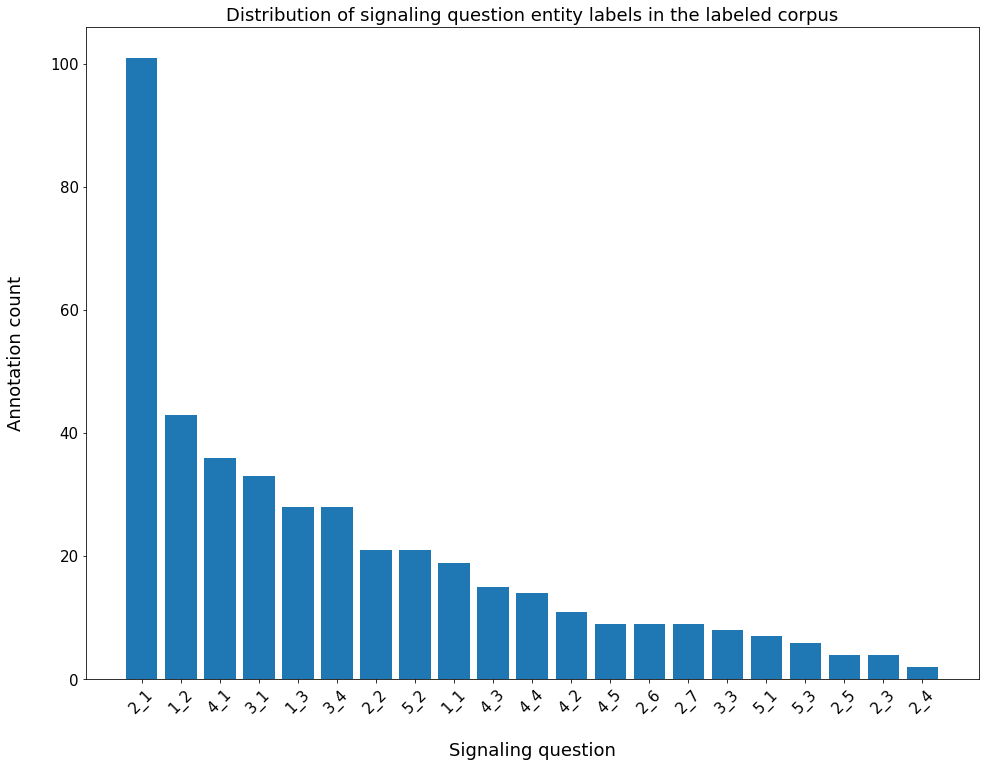
\includegraphics[width=0.60\columnwidth]{figures/rob_annot_freq.png}
    \caption{Total number of annotations made for each signalling question.}
    \label{fig:flowchart}
\end{figure}
%
%
%


\begin{table}[htb]
    \centering
    \caption{General statistics for the annotated corpus}
    \label{table:stats}
    \begin{tabular}{lrrrrr}
    \hline
         Signalling Question & Total tokens & Mean tokens & Average length & Total documents \\ \hline
        RoB 1.1 & 0 & 0 & 0 & 0 \\ 
        RoB 1.2 & 0 & 0 & 0 & 0 \\ 
        RoB 1.3 & 0 & 0 & 0 & 0 \\ 
        RoB 2.1 & 0 & 0 & 0 & 0 \\ 
        RoB 2.2 & 0 & 0 & 0 & 0 \\ 
        RoB 2.3 & 0 & 0 & 0 & 0 \\ 
        RoB 2.4 & 0 & 0 & 0 & 0 \\ 
        RoB 2.5 & 0 & 0 & 0 & 0 \\ 
        RoB 2.6 & 0 & 0 & 0 & 0 \\ 
        RoB 2.7 & 0 & 0 & 0 & 0 \\ 
        RoB 3.1 & 0 & 0 & 0 & 0 \\ 
        RoB 3.2 & 0 & 0 & 0 & 0 \\ 
        RoB 3.3 & 0 & 0 & 0 & 0 \\ 
        RoB 3.4 & 0 & 0 & 0 & 0 \\ 
        RoB 4.1 & 0 & 0 & 0 & 0 \\ 
        RoB 4.2 & 0 & 0 & 0 & 0 \\ 
        RoB 4.3 & 0 & 0 & 0 & 0 \\ 
        RoB 4.4 & 0 & 0 & 0 & 0 \\ 
        RoB 4.5 & 0 & 0 & 0 & 0 \\ 
        RoB 5.1 & 0 & 0 & 0 & 0 \\ 
        RoB 5.2 & 0 & 0 & 0 & 0 \\ 
        RoB 5.3 & 0 & 0 & 0 & 0 \\ \hline
    \end{tabular}
\end{table}
%
%
%
\subsection{Inter-annotator agreement}
%
Table \ref{table:IAA_sq} illustrates the levels of inter-annotator agreement between the two consensus annotators, both before and after the development of the guidelines.
%
%
%
\begin{table}[htb]
    \caption{IAA before after visual placards development}
    \label{table:IAA_sq}
    \centering
    \begin{tabular}{llll}
    \hline
        Signalling question & before guideline improvement & after guidelines improvement & change \\
    \hline
        RoB 1\_1 & 24.44 & 55.02 & +30.58 \\ 
        RoB 1\_2 & 50.28 & 44 & -6.28 \\ 
        RoB 1\_3 & 20.44 & 90.9 & +70.46 \\ 
        RoB 2\_1 & 1.34 & 67.26 & +65.92 \\ 
        RoB 2\_2 & 7.23 & 38.66 & +31.43 \\ 
        RoB 2\_3 & 5.42 & 0 & -5.42 \\ 
        RoB 2\_4 & - & 0 & 0 \\ 
        RoB 2\_5 & 0 & 0 & 0 \\ 
        RoB 2\_6 & 68.85 & 83.25 & +14.4 \\ 
        RoB 2\_7 & 6.52 & 0 & -6.52 \\ 
        RoB 3\_1 & 23.57 & 39.68 & +16.11 \\ 
        RoB 3\_2 & 0 & ~ & 0 \\ 
        RoB 3\_3 & 0 & 0 & 0 \\ 
        RoB 3\_4 & 0 & 0 & 0 \\ 
        RoB 4\_1 & 6.51 & 61.71 & +55.2 \\ 
        RoB 4\_2 & 0 & 0 & 0 \\ 
        RoB 4\_3 & 13.85 & 30.21 & +16.36 \\ 
        RoB 4\_4 & 0 & 56.25 & +56.25 \\ 
        RoB 4\_5 & 0 & 0 & 0 \\ 
        RoB 5\_1 & 0 & 0 & 0 \\ 
        RoB 5\_2 & 0 & 49.49 & +49.49 \\ 
        RoB 5\_3 & 0 & 0 & 0 \\ \hline
    \end{tabular}
\end{table}
%
%
%
\subsection{LLM evaluation}
%
XoX


\begin{table}[htb]
    \caption{LLM accuracy}
    \label{table:LLM_eval}
    \centering
    \begin{tabular}{llll}
    \hline
        Signalling question & Simple prompts & Detailed prompts & change \\
    \hline
        RoB 1\_1 & 24.44 & 55.02 & +30.58 \\ 
        RoB 1\_2 & 50.28 & 44 & -6.28 \\ 
        RoB 1\_3 & 20.44 & 90.9 & +70.46 \\ 
        RoB 2\_1 & 1.34 & 67.26 & +65.92 \\ 
        RoB 2\_2 & 7.23 & 38.66 & +31.43 \\ 
        RoB 2\_3 & 5.42 & 0 & -5.42 \\ 
        RoB 2\_4 & - & 0 & 0 \\ 
        RoB 2\_5 & 0 & 0 & 0 \\ 
        RoB 2\_6 & 68.85 & 83.25 & +14.4 \\ 
        RoB 2\_7 & 6.52 & 0 & -6.52 \\ 
        RoB 3\_1 & 23.57 & 39.68 & +16.11 \\ 
        RoB 3\_2 & 0 & ~ & 0 \\ 
        RoB 3\_3 & 0 & 0 & 0 \\ 
        RoB 3\_4 & 0 & 0 & 0 \\ 
        RoB 4\_1 & 6.51 & 61.71 & +55.2 \\ 
        RoB 4\_2 & 0 & 0 & 0 \\ 
        RoB 4\_3 & 13.85 & 30.21 & +16.36 \\ 
        RoB 4\_4 & 0 & 56.25 & +56.25 \\ 
        RoB 4\_5 & 0 & 0 & 0 \\ 
        RoB 5\_1 & 0 & 0 & 0 \\ 
        RoB 5\_2 & 0 & 49.49 & +49.49 \\ 
        RoB 5\_3 & 0 & 0 & 0 \\ \hline
    \end{tabular}
\end{table}
%
%
%
\section{Discussion}
\label{sec:discussion}
%
After the first batch of documents (n=9) was annotated and the F1 measure IAA calculated, we saw some questions had zero agreement.
Our aim was to use the annotated corpus and resolve the conflicts between the annotators to increase the annotation agreement and also improve the instructions in the placards.
For multiple conflicting cases, the instructions were either unclear, interpreted differently, or the annotators forgot to annotate.
However, when the annotators went through the conflicts, they were able to resolve them.
Therefore, we recommend semi-automation for RoB information extraction given two succinct reasons.
Reason 1: Cognitive load of annotating (and assessment). Machine learning models can help function like ``hint finding'' for many questions.
Reason 2: Subjective judgments within the signalling questions.
~\cite{loef2022interrater}


%
%
%
\subsection{Conflict resolution}
%
During conflict resolution, we found that certain instances where both annotators marked the same text evidence to answer the same SQ but gave different .
We resorted to face-to-face conflict resolution in this case for every conflict case and updated the visual placards.
We went for conflict resolution in the scenarios when
1) the annotators marked different parts of text to answer the same question with same judgment. (\url{https://docs.google.com/spreadsheets/d/14jYqXTcnVzZsC5pbKQ2GcwtVrwl81DG9Yo5uhCJZzjo/edit#gid=1107412538})
2) the annotators marked same part of text to answer the same question, but gave different judgment option for it. (\url{https://docs.google.com/spreadsheets/d/14jYqXTcnVzZsC5pbKQ2GcwtVrwl81DG9Yo5uhCJZzjo/edit#gid=0})
Both annotators use different parts of text to answer the same signalling question, but give different judgment options. \url{https://docs.google.com/spreadsheets/d/14jYqXTcnVzZsC5pbKQ2GcwtVrwl81DG9Yo5uhCJZzjo/edit#gid=1107412538}
In case, one annotator selected a part of text and another the same text but an additional text too, then we will select the annotations from the longer annotation.
%
%
%
\subsection{LLM evaluation}
\label{disc:llm}
%
We had a few examples where ChatPDF generated an answer to the signalling question, but these sentences comprising the answer were not to be found in the input PDF document.
After instructing ChatPDF to look into the uploaded PDF and not generate sentences by itself, it gives the following output.
``I apologize, but as an AI language model, I do not have access to any uploaded PDFs or any external sources. Please provide me with the PDF you are referring to, and I will be happy to extract the sentences related to answering the signalling question RoB 1.1.''
When no information was found to answer a RoB question, ChatPDF generates a response by itself giving example sentences that could be used to answer that question.
Can retrieve multiple related answers for a RoB question prompt and one of that has to be the correct answer and should be the same as what the annotators annotated.
%
%
%
\subsection{Limitations}
\label{subsec:limits}
%
Our study has the following limitations.
Firstly, a limitation arises from the relatively small scale of our annotations, with only 60 documents undergoing the annotation process.
This constraint is primarily due to financial constraints, as the availability of funds limited our ability to hire a larger number of expert annotators.
%Despite this limitation, the robustness of the annotations provided by the experts remains noteworthy, as they diligently scrutinized the selected documents within the resources at hand.
A second limitation stems from the narrow focus of annotations, concentrated exclusively on physiotherapy and rehabilitation clinical trials.
This specificity arises from our reliance on domain experts for annotations, who possess the requisite expertise in these areas. While this targeted approach guarantees high-quality annotations within the specified domains, it inadvertently restricts the broader applicability of the annotated corpus.
%Nonetheless, the in-depth and accurate annotations derived from expert knowledge substantially contribute to the reliability of the study's outcomes within the designated domains.
Thirdly, our study's scope is delimited by the selection of particular journals to construct the corpus in addition to certain RCTs selected randomly.
This choice was necessitated by the desire to incorporate articles of the utmost quality, ensuring the inclusion of high-caliber research in the analysis.
While this decision ensures a certain standard of literature, it inadvertently excludes a wider spectrum of articles, potentially biasing the corpus toward a specific subset of clinical trials. It's important to note that the chosen journals might have their own editorial policies, thereby limiting the diversity of included studies.
This methodological trade-off, while benefiting the corpus's overall quality, might inadvertently influence the representation of risk of bias annotations, particularly in relation to lower quality trials.

%
%
%
\section{Conclusion}
\label{sec:conclusion}
%
We have presented RoBuster: a new, publicly-available corpus, comprising 60 full-text randomized controlled trials richly annotated with 22 signalling questions.
The dataset fills a need for a corpus to evaluate risk of bias span extraction using machine learning technologies.
Our corpus has detailed and fine-grained information in form of individual risk of bias spans along with annotator decision on the bias risk (high or low).
As it has been developed by bias assessors and natural language processing experts, RoBuster can support automated approaches to bias assessment and can also be a part SLR (living systematic review) systems.
Throughout our journey, we've encountered several challenges during RoB annotation. These experiences have led us to outline refinements in the discussion section, offering insights to guide future studies in this domain.
In the future, we plan to extend this corpus by adding more annotated full-texts.
%In addition, LLMs could be fine-tuned with the available annotations to further refine the corpus with new annotations which could have been missed.
Another direction to test whether the developed visual placards could be used to train fresh risk of bias assessors.
%
%
%
\section{Abbreviations}%% if any
%
\begin{enumerate}
    \item RCT - Randomized Controlled Trial
    \item RoB - Risk of Bias
    \item SR - Systematic review
    \item SQ - Signalling Question
    \item LLM - Large Language Model
    \item GPT - Generative Pre-trained Transformer
    \item NLP - Natural Language Processing
    \item IAA - Inter-annotator Agreement
    \item PEDro - Physiotherapy Evidence Database RoB scale
    \item AMSTAR - A MeaSurement Tool to Assess systematic Reviews - Risk of Bias
    \item EPOC RoB - Effective Practice and Organisation of Care - Risk of Bias tool
    \item CDSR - Cochrane Database of Systematic Reviews
\end{enumerate}
%
%
%
\backmatter

\bmhead{Supplementary information}
%
The visual placards along with detailed annotation instructions, the RCTs used in this study along with their license information, and an extended discussion section are included in the supplementary information files.
%
%
%
\bmhead{Acknowledgments}

%Acknowledgements are not compulsory. Where included, they should be brief. Grant or contribution numbers may be acknowledged.

%Please refer to Journal-level guidance for any specific requirements.
This research was supported by HES-SO, Valais-Wallis. 

%
%
%
\section*{Declarations}
%
\subsection*{Funding}
%
This research was supported by HES-SO, Valais-Wallis, Sierre, Switzerland. 
%
%
%
\subsection*{Conflict of interest}
%
The authors declare that they have no competing interests.
%
%
%
\subsection*{Competing interest}
%
The authors declare that they have no competing interests.
%
%
%
%\subsection*{Ethics approval}
%
%Not applicable
%
%
%
\subsection*{Consent to participate and publish}
%
The experts who undertook the visual placards development and the annotation process for this corpus were explained the purpose of the annotation project and agreed to voluntarily participate in the study.
Even though they agreed to participate in the study, they can withdraw their participation any time without consequences of any kind.
They were explained the purpose and nature of the study in form of a presentation and had an opportunity to ask questions.
They were also fully informed about the purpose of the study and the eventual publication of the findings.
Each expert provided explicit consent for the publication of the annotated corpus, along with the understanding that any identifying information would be appropriately anonymized to protect their privacy. 
%
%
%
\subsection*{Data availability}
%
Availability of data and materials on the journals preferred portal.
%
%
%
\subsection*{Code availability}
%
The notebooks used analyze the corpus will be available on GitHub.
%
%
%
%\subsection*{Authors' contributions}
%
%Authors' contributions
%BMC journals: \url{https://www.biomedcentral.com/getpublished/editorial-policies}
%
%
%
%%===================================================%%
%% For presentation purpose, we have included        %%
%% \bigskip command. please ignore this.             %%
%%===================================================%%
%
\begin{appendices}
%
%
%
\section{Annotation guidelines}\label{annot_guidelines}
%
An appendix contains supplementary information that is not an essential part of the text itself but which may be helpful in providing a more comprehensive understanding of the research problem or it is information that is too cumbersome to be included in the body of the paper.
%
%
%
\end{appendices}

%%===========================================================================================%%
%% If you are submitting to one of the Nature Portfolio journals, using the eJP submission   %%
%% system, please include the references within the manuscript file itself. You may do this  %%
%% by copying the reference list from your .bbl file, paste it into the main manuscript .tex %%
%% file, and delete the associated \verb+\bibliography+ commands.                            %%
%%===========================================================================================%%

\bibliography{bibliography.bib}% common bib file
%% if required, the content of .bbl file can be included here once bbl is generated
%%\input sn-article.bbl


\end{document}
